\documentclass[12pt,a4paper,oneside,english]{book}

\usepackage{cite}

\usepackage[T1]{fontenc}
\usepackage[english]{babel}
\usepackage{amsmath}
\usepackage{amsfonts}
\usepackage{amssymb}
\usepackage{graphicx}
\usepackage{subfig}
\usepackage{fancyhdr}
\usepackage{appendix}
\usepackage{hyphenat}
\usepackage{pdfpages}
\usepackage{etoc}
\usepackage{minitoc}
\usepackage{lipsum}
\usepackage{natbib}
\usepackage{float}
\usepackage{svg}
\usepackage{amsthm}


%\usepackage{newtxtext}  % For text
%\usepackage{newtxmath}  % For consistent math fonts
\newtheorem{theorem}{Theorem}
\newtheorem{corollary}{Corollary}
\newtheorem{lemma}{Lemma}
\newtheorem{proposition}{Proposition}


\usepackage{array,multirow,makecell}
\newcolumntype{C}[1]{>{\arraybackslash}p{#1}}

\usepackage{enumitem}
\setlist{leftmargin=*,itemsep=0pt}

\usepackage{centernot}
\usepackage[linesnumbered,ruled,vlined,english,onelanguage]{algorithm2e}

\usepackage{quotchap}
\makeatletter
\renewcommand{\@makechapterhead}[1]{
 \chapterheadstartvskip
 {\size@chapter{\sectfont\raggedright
 {\chapnumfont
 \ifnum \c@secnumdepth >\m@ne
 \if@mainmatter\thechapter
 \fi\fi
 \par\nobreak}
 {\raggedright\advance\leftmargin10em\interlinepenalty\@M #1\par}}
 \nobreak\chapterheadendvskip}}
\makeatother
\renewcommand*{\chapterheadendvskip}{\vspace{2cm}}

\usepackage{geometry}
\geometry{hmargin=2.5cm,vmargin=2.5cm}

\pagestyle{fancyplain}
\lhead{\fancyplain{}{\nouppercase{\textit{\leftmark}}}}
\chead{\fancyplain{}{}}
\rhead{\fancyplain{}{}}
\lfoot{\fancyplain{}{}}
\cfoot{\fancyplain{}{}}
\rfoot{\fancyplain{\thepage}{\thepage}}
\renewcommand{\headrulewidth}{1pt}
\renewcommand{\footrulewidth}{1pt}

\renewcommand{\thesection}{\arabic{section}}

\usepackage{titlesec}
\titleformat{\paragraph}{\fontsize{11}{10}\bfseries}{\theparagraph}{1em}{}
\titlespacing*{\paragraph}{0pt}{10pt plus 2pt minus 0pt}{0pt plus 2pt minus 0pt}

\setcounter{secnumdepth}{4}
\setcounter{tocdepth}{4}

\usepackage{array}
\usepackage{multirow}
%\addto\captionsfrench{\def\tablename{\textsc{Tableau}}}

%\DefineBibliographyStrings{french}{urlseen = {},}

\setlength{\parskip}{8pt}
\usepackage{setspace}

\usepackage{url}

\usepackage{hyperref}
% Comment before printing to remove links' colors
\definecolor{darkblue}{rgb}{0.0, 0.0, 0.5}
\hypersetup{
 colorlinks,
 linktocpage=true,
 linkcolor={darkblue},
 citecolor={darkblue},
 urlcolor={blue}}

\sloppy

\author{You}
\title{Rapport de PFA RT4}




\makeatletter
\def\@pnumwidth{2em}   % Space reserved for page numbers
\def\@tocrmarg{3.5em}  % Right margin for TOC entries
\makeatother


\begin{document}
\pagenumbering{gobble}
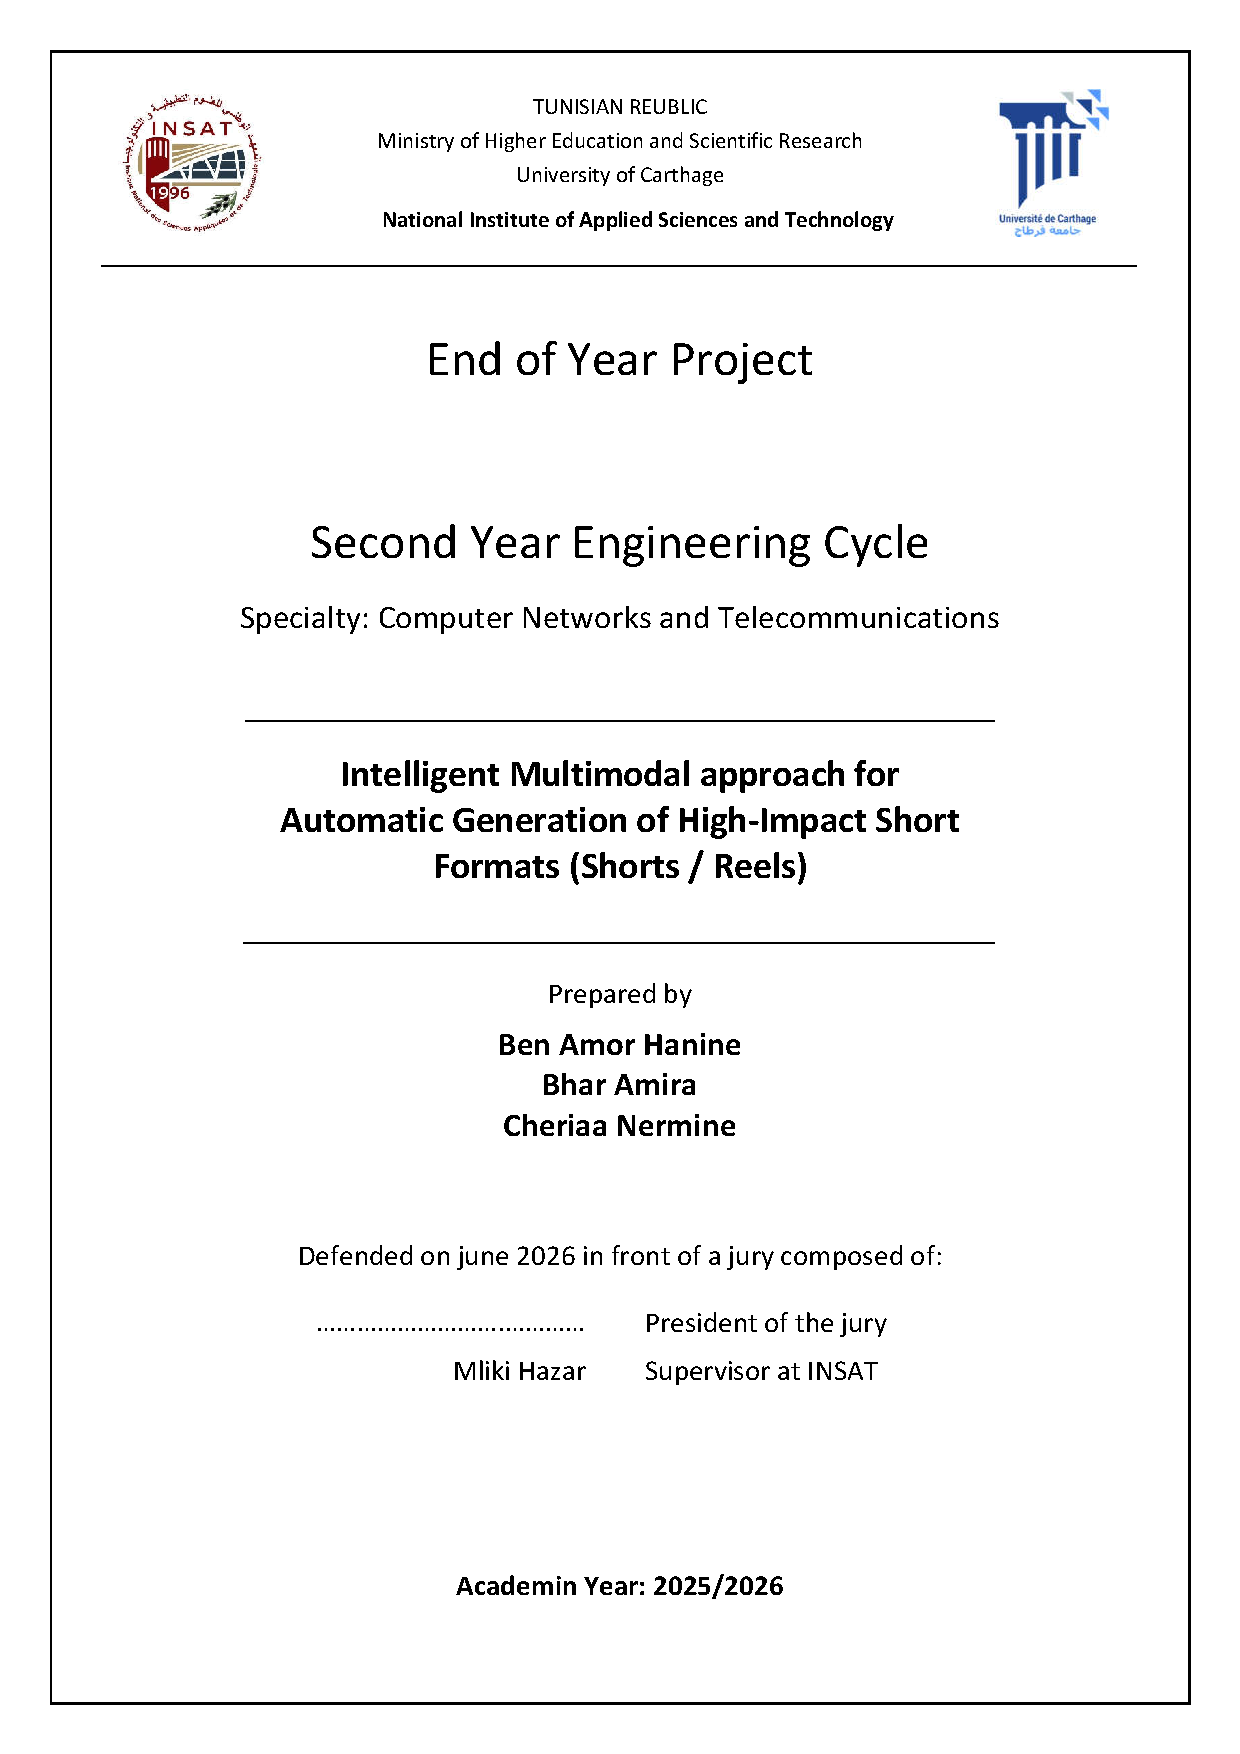
\includepdf[pages=-]{FrontPage.pdf}
\chapter*{Acknowledgments}

\frontmatter
\chapter*{Abstract}
\normalsize{Write your abstract here}.

\medskip
{\noindent \textbf{Keywords: ..., ... .} }

\spacing{1}
\tableofcontents{}
\newpage 
\listoffigures
\newpage 
\listoftables
\newpage
\spacing{1.4}
\chapter*{List of acronyms}
%\addcontentsline{toc}{chapter}{Liste des acronymes}
\markboth{List of acronyms}{}
\begin{itemize}
\item \textbf{Abbrev.} Abbreviation
\end{itemize}

\mainmatter
%\mtcaddchapter[Introduction g�n�rale] 
\chapter*{Introduction}
\addcontentsline{toc}{chapter}{Introduction}
\markboth{Introduction}{}
%besoin+probleme+ solution+steps+overview of the report
azerty



\mainmatter
\chapter{State of the Art}
\label{ch:state_of_the_art}

%models available and their key concepts
%souel: el relevance of the 3 modalitites comment nahkiw aliha?
 % unnumbered - just contextual paragraph %hanine
 \section*{Introduction}
\section{Unimodal Approaches for Video Understanding}%amira
% Conceptual section: what is unimodal, why it's limited

\subsection{Visual Understanding}
% Frame-level analysis, optical flow, scene detection

\subsection{Audio Understanding}
% Acoustic features, spectral analysis, speech processing

\subsection{Textual Understanding}
% NLP for transcripts, sentiment, keyword extraction

\section{Representative Unimodal Models and Frameworks}
\subsection{Whisper}     % ASR- you use this
\subsection{Librosa}     % Audio features - you use this
\subsection{OpenCV / Decord}  % Video frame extraction - you use this

\section{Fusion-Based Multimodal Systems}
% Conceptual section: early/late/hybrid fusion
% Limitations of fusion without joint training

\section{Joint Multimodal Representation Learning}%hanine
% Conceptual section: contrastive learning, shared embedding spaces
% CLIP paradigm, temperature scaling, zero-shot transfer
Joint multimodal representation learning addresses a fundamental limitation shared by both unimodal and fusion-based approaches: the absence of a unified semantic space in which modalities such as vision, audio, and text can be collectively  treated and compared. 
Rather than processing each signal independently and combining outputs,the joint approach  trains a single model to map all modalities into a shared high-dimensional embedding space, where geometric proximity reflects semantic similarity regardless of the originating modality.
\\Modern multimodal systems are inspired by the contrastive learning framework popularized by CLIP-like architectures, enabling cross-modal reasoning where heterogeneous modalities are treated as different expressions of the same underlying objective.

\subsection{Contrastive Learning Framework}

\subsection{Shared Embedding Spaces}

\subsection{Zero-Shot Transfer and Cross-Modal Retrieval}

\subsection{Advantages of Joint Multimodal Learning}

\subsection{Limitations and Challenges}



\section{Representative Multimodal Models}
%https://encord.com/blog/top-multimodal-models/

\subsection{CLIP}%amira
\subsection{AudioCLIP or CLAP}   % hanine
\subsection{Flamingo }%nermine
The Flamingo model developed by DeepMind is a powerful family of Visual Language Models designed to process sequences of images or videos
interleaved with text and generate free-form text as output. \\
Flamingo represents a notable progression in vision-language modeling by enabling a single model to perform multiple multimodal tasks with minimal task-specific fine-tuning.

A core concept of its architecture is the fusion of large, pre-trained, and frozen models specifically a \textbf{vision encoder} and a \textbf{language model}—to leverage their existing knowledge without the need for intensive retraining . \\To efficiently bridge these two modalities, Flamingo introduces \textbf{the Perceiver Resampler}, which compresses a huge number of visual features into a fixed-size collection of visual tokens , these tokens then condition the frozen language model through \textbf{Gated Cross-Attention layers}, which are interleaved between the original language model layers , these gated layers are essential for preserving the stability of the model during training and ensuring the language model's original performance remains intact at initialization.

A key contribution of Flamingo is its \textbf{few-shot learning} capability The model can adapt to various tasks with only a few input-output examples .
Experimental evaluations showed strong performance across several vision–language benchmarks,  such as multimodal reasoning tasks, visual question answering and image captioning .


\subsection{LLAVA}%nermine
LLaVA  is a multimodal model designed to enhance general-purpose visual and language understanding through the use of visual instruction tuning 

The architecture of LLaVA  consists of a \textbf{pretrained CLIP  vision encoder }and a \textbf{Vicuna large language model}, which are connected by a two-layer \textbf{Multi-Layer Perceptron cross-modal projector} .\\
This MLP projector converts visual encoder tokens into post-embedding layer LLM tokens, replacing the simpler linear projection used in earlier versions to improve multimodal capabilities .\\
The training process follows a \textbf{two-stage pipeline:} an initial stage focused on modality alignment using roughly 600,000 image-text pairs, followed by a second stage of visual instruction fine-tuning where the model is trained on diverse conversation datasets .\\
This approach enables LLaVA to perform tasks such as image description, visual question answering, and multimodal dialogue generation. Compared to more complex architectures, LLaVA is considered more accessible and computationally efficient while maintaining competitive performance.
\subsection{Video-LLaMA} % hanine
\subsection{ImageBind}%amira   
% Last = most important
\section{Comparative Analysis and Discussion} %hanine
% Table comparing all models across key criteria
% Quantitative where possible (params, modalities, zero-shot, etc.)

\section{Positioning of the Proposed Approach}% hanine
% Justification of selected paradigm
% Justification of selected model family

%+ Bridge to Chapter 2 (Methodology)



\section*{Conclusion}

\chapter*{Conclusion and perspectives}
\addcontentsline{toc}{chapter}{Conclusion and perspectives}
\markboth{Conclusion and perspectives}{}

\begin{appendix}
\chapter{Appendix 1}
Insert your appendixes here if you need.
\end{appendix}

%\spacing{1}
\bibliographystyle{unsrt}
\bibliography{references}
\end{document}
